\documentclass[12pt,a4paper]{article}
\usepackage{amsmath,amscd,amsbsy,amssymb,latexsym,url,bm,amsthm}
\usepackage{epsfig,graphicx,subfigure}
\usepackage{enumitem,balance}
\usepackage{wrapfig}
\usepackage{mathrsfs,euscript}
\usepackage[usenames]{xcolor}
\usepackage{hyperref}
\usepackage[vlined,ruled,linesnumbered]{algorithm2e}
\usepackage{array}
\usepackage{float}
\hypersetup{colorlinks=true,linkcolor=black}
\usepackage{attachfile}
\usepackage{listings}

\newtheorem{theorem}{Theorem}
\newtheorem{lemma}[theorem]{Lemma}
\newtheorem{proposition}[theorem]{Proposition}
\newtheorem{corollary}[theorem]{Corollary}
\newtheorem{exercise}{Exercise}
\newtheorem*{solution}{Solution}
\newtheorem{definition}{Definition}
\theoremstyle{definition}

\renewcommand{\thefootnote}{\fnsymbol{footnote}}

\newcommand{\postscript}[2]
 {\setlength{\epsfxsize}{#2\hsize}
  \centerline{\epsfbox{#1}}}

\renewcommand{\baselinestretch}{1.0}

\setlength{\oddsidemargin}{-0.365in}
\setlength{\evensidemargin}{-0.365in}
\setlength{\topmargin}{-0.3in}
\setlength{\headheight}{0in}
\setlength{\headsep}{0in}
\setlength{\textheight}{10.1in}
\setlength{\textwidth}{7in}
\makeatletter \renewenvironment{proof}[1][Proof] {\par\pushQED{\qed}\normalfont\topsep6\p@\@plus6\p@\relax\trivlist\item[\hskip\labelsep\bfseries#1\@addpunct{.}]\ignorespaces}{\popQED\endtrivlist\@endpefalse} \makeatother
\makeatletter
\renewenvironment{solution}[1][Solution] {\par\pushQED{\qed}\normalfont\topsep6\p@\@plus6\p@\relax\trivlist\item[\hskip\labelsep\bfseries#1\@addpunct{.}]\ignorespaces}{\popQED\endtrivlist\@endpefalse} \makeatother

\begin{document}
\noindent

%========================================================================
\noindent\framebox[\linewidth]{\shortstack[c]{
\Large{\textbf{Lab06-Linear Programming}}\vspace{1mm}\\
CS214-Algorithm and Complexity, Xiaofeng Gao, Spring 2021.}}
\begin{center}
\footnotesize{\color{red}$*$ If there is any problem, please contact TA Haolin Zhou.}

% Please write down your name, student id and email.
\footnotesize{\color{blue}$*$ Name: Beichen Yu  \quad Student ID: 519030910245 \quad Email: polarisybc@sjtu.edu.cn}
\end{center}

\begin{enumerate}
    \item
    \textit{Hirschberg Algorithm.} Recall the \textbf{String Similarity} problem in class, in which we calculate the edit distance between two strings in a sequence alignment manner.
    \begin{enumerate}
    	\item
    	Implement the algorithm combining \textbf{dynamic programming} and \textbf{divide-and-conquer} strategy in C/C++. Analyze the time complexity of your algorithm. {\color{blue}(The template \emph{Code-SequenceAlignment.cpp} is attached on the course webpage)}.
    	
    	\item
    	Given $\alpha(x, y) = |ascii(x) - acsii(y)|$, where $ascii(c)$ is the ASCII code of character $c$, and $\delta=13$. Find the edit distance between the following two strings.
    	\begin{align*}
    		X[1..60]=&\ CMQHZZRIQOQJOCFPRWOUXXCEMYSWUJ\\
    		&\ TAQBKAJIETSJPWUPMZLNLOMOZNLTLQ	
    	\end{align*}
    	\begin{align*}
    		Y[1..50]=&\ SUYLVMUSDROFBXUDCOHAATBKN\\
    		&\ AAENXEVWNLMYUQRPEOCJOCIMZ
    	\end{align*}
    \end{enumerate}
    
    \begin{solution}
    \begin{enumerate}
    \item	The code is included in the .zip file.
    Denote $T(m,n)$ as the max running time of algorithm on strings of length $m$ and $n$. To compute $f(\cdot,n/2)$ and $g(\cdot,n/2)$, and find the middle index $q$ at the same time, we need $O(mn)$ time. So we have:
    $$T(m,n) \leqslant cmn + T(q,n/2) + T(m-q,n/2)$$
    
    Now we consider the base cases. If $m = 2$, we have $T(2,n) \leqslant cn$; At the same time, if $n = 2$, we have $T(m,2) \leqslant cm$. 
    
    Using the strong induction, we assume that if $i \leqslant m$ and $j \leqslant n$, $T(i,j) \leqslant 2cij$. Then we have:
   	\begin{align*}
   	T(m,n) &\leqslant cmn + T(q,n/2) + T(m-q,n/2)\\
   	&\leqslant cmn + 2c \cdot q \cdot n/2 + 2c \cdot (m-q) \cdot n/2 \\
   	&= cmn + cqn + cmn - cqn\\
   	&= 2cmn
   	\end{align*}
   	
   	That means the time complexity of this algorithm is $O(mn)$.
   	
   	\item
   	
    I created the "X.txt" and "Y.txt" files, and copied the sequences X and Y into them. Then through running \emph{Code-SequenceAlignment.cpp}, I got the answer 385. Below is the result of my program.
   	\begin{figure}[H]
    \centering
    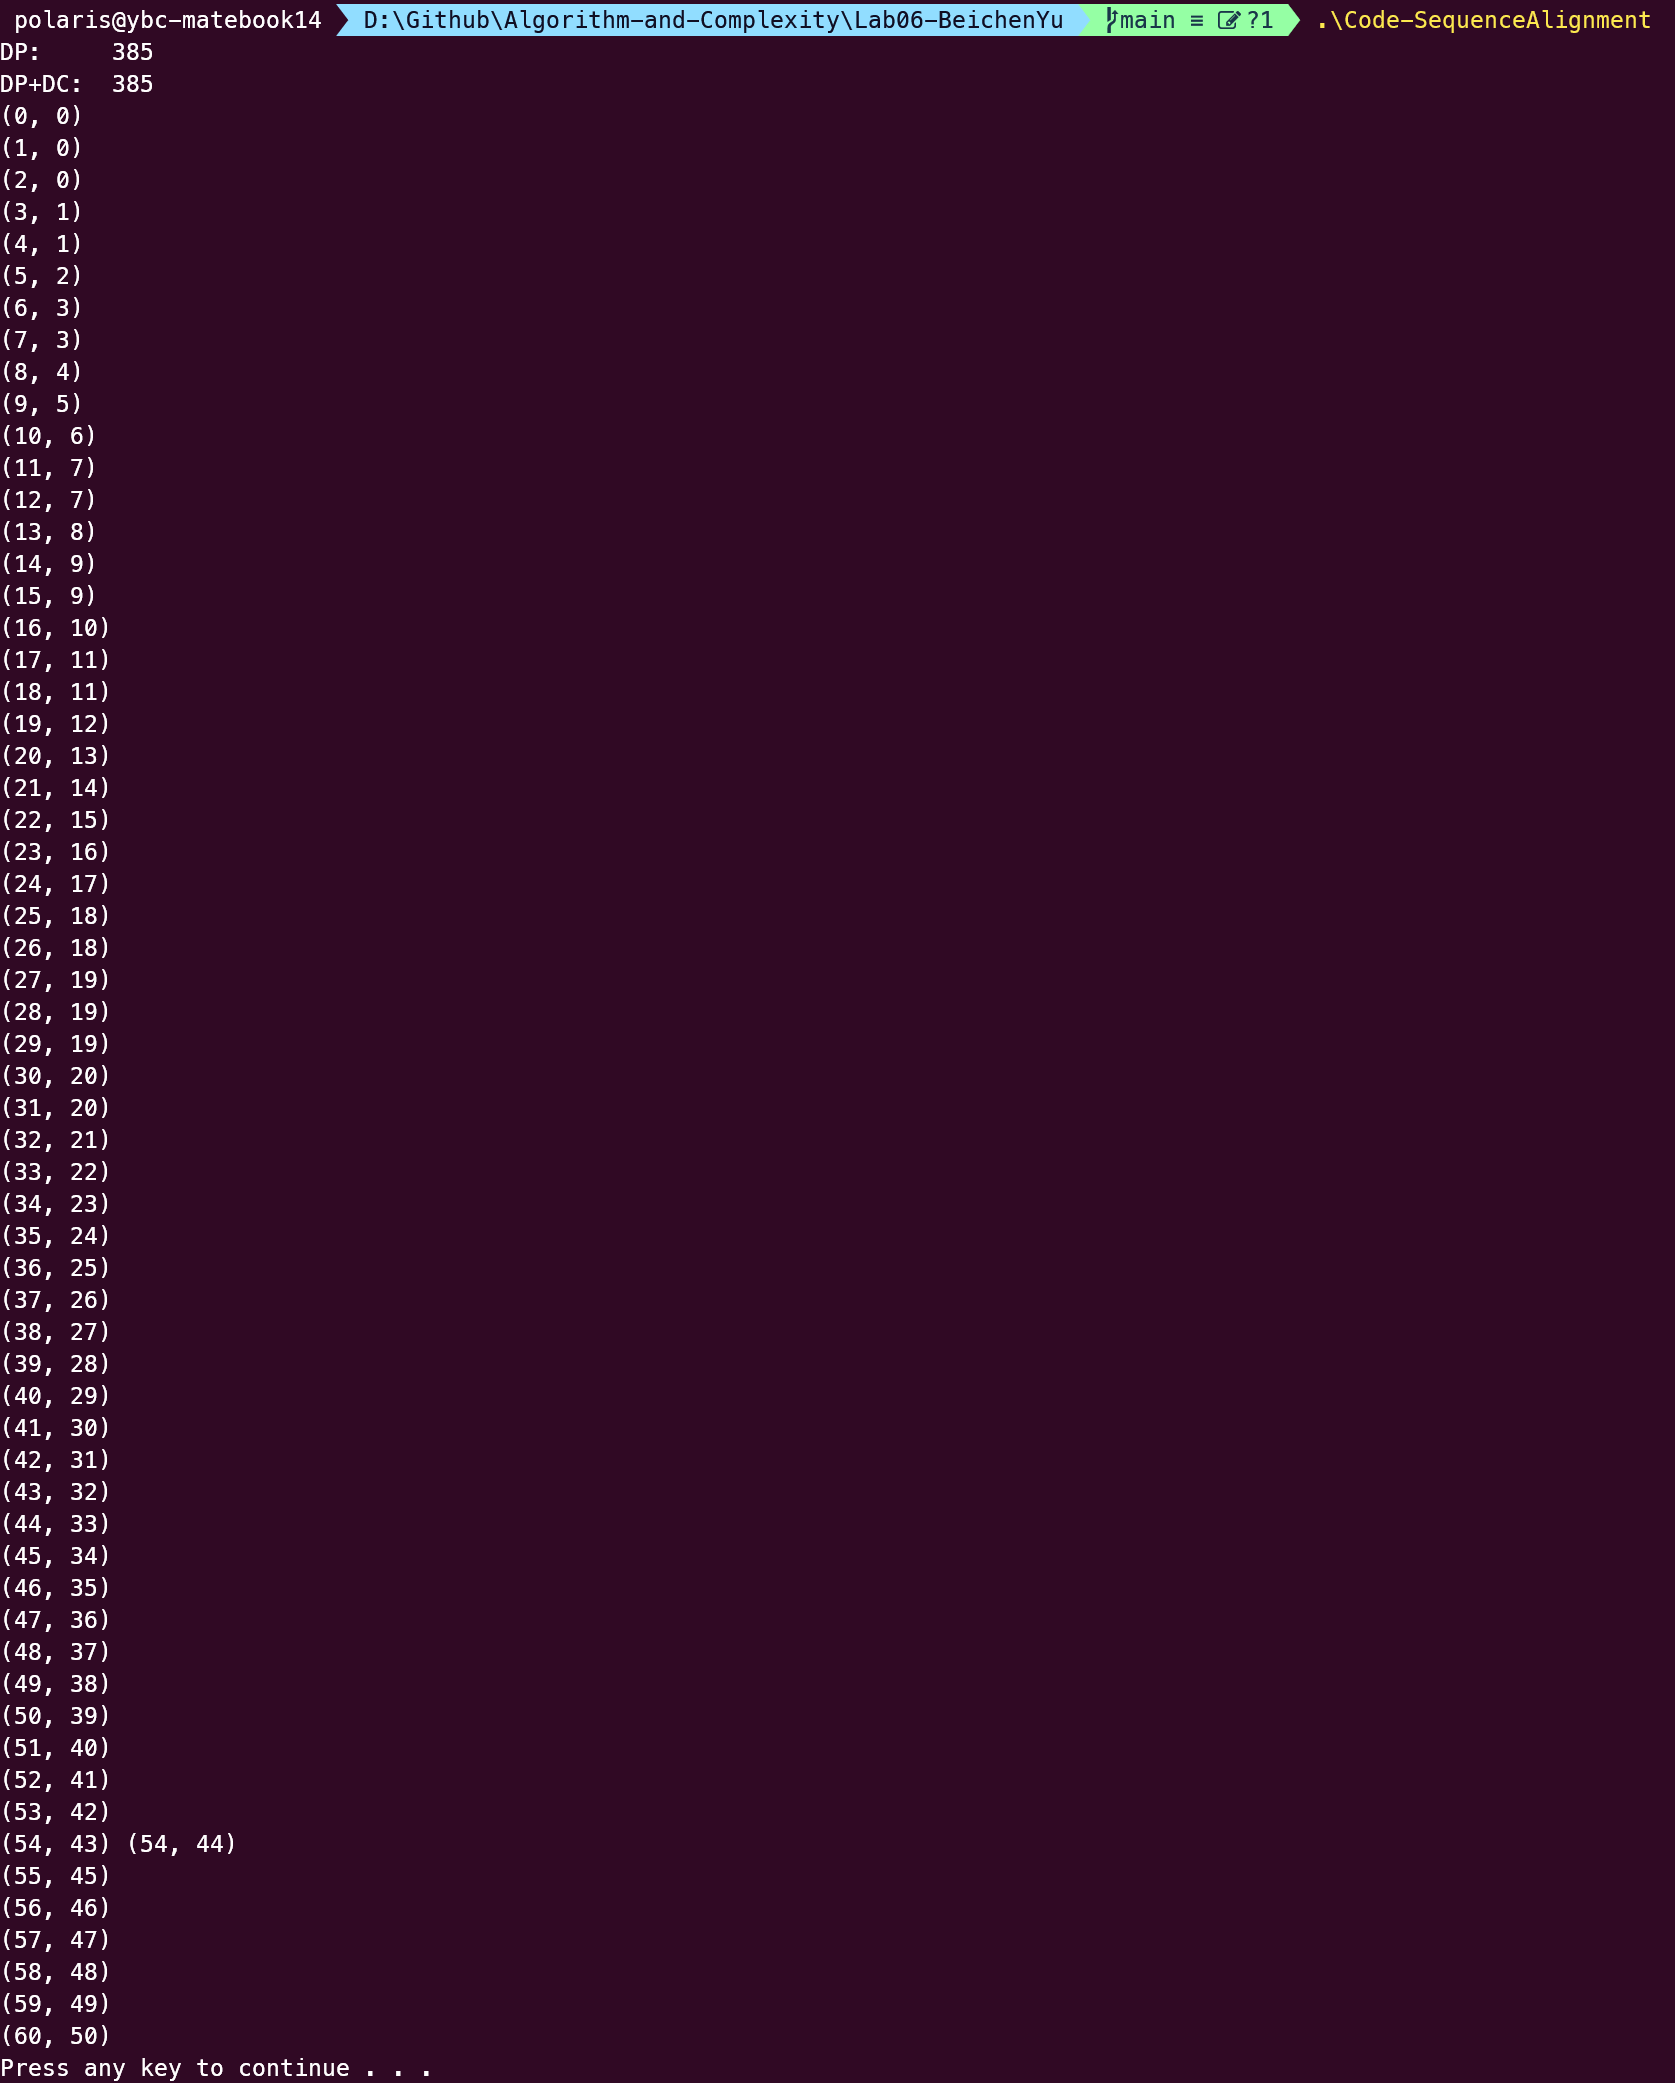
\includegraphics[width=0.5\textwidth]{sequence.png}
    \caption{The result of the program}
\end{figure}
    \end{enumerate}
    \end{solution}
    
    
    
    \item 
    \textit{Travelling Salesman Problem.} Given a list of cities and the distances between each pair of cities ($ G=(V,E,W) $), we want to find the shortest possible route that visits each city exactly once and returns to the origin city. Similar to \textbf{Maximum Independent Set} and \textbf{Dominating Set}, please turn the traveling salesman problem into an ILP form.  
    
    \textbf{Remark:} $ W $ is the set of weights corresponds to the edges that connecting adjacent cities.  
    
    
    \begin{solution}
    
    Denote $x_{ij}$ as whether the edge $e_{ij}$ is selected by the salesman. 
    
    To make it clearer, we first denote $I$ as the edges selected by the salesman, then we have:
    
    $$ x_{ij}=\left\{
	\begin{aligned}
	1, x_{ij} \in I\\
	0, x_{ij} \notin I
	\end{aligned}
	\right.
	$$
	
	Obviously we need to minimize $\sum_{i,j}w_{ij}x_{ij}$.
	
	Then let us find the constraints:
	
	\begin{enumerate}
	\item All of the vertexes are reached by the salesman. That means for every vertex, the in-degree and the out-degree are both 1. Assume that there are $n$ vertexes, we have:
	$$\sum^{n}_{i=1,i \neq j} x_{ij} = 1, j = 1,2,\cdots,n$$
	$$\sum^{n}_{j=1,i \neq j} x_{ij} = 1, i = 1,2,\cdots,n$$
	\item We need that there is no sub-loop in $I$. In a sub-loop $S$, we find that $\sum_{i,j \in S} x_{ij} = |S|$. So we need to add the  constraint:
	$$\sum_{i,j \in S} x_{ij} \leqslant |S| - 1, \forall S \subseteq V, 1 < |S| < n$$
	\end{enumerate}
	
	Above all, we can rewrite the traveling salesman problem into below ILP form:
	
	
	$$min  \quad \sum^{n}_{i = 0}\sum^{n}_{j \neq i, j = 0} w_{ij}x_{ij}$$
	\begin{align*}
	s.t. &\quad 0 \leqslant x_{ij} \leqslant 1 \qquad i,j = 1,2,\cdots,n\\
	&\sum^{n}_{i=1,i \neq j} x_{ij} = 1  \qquad j = 1,2,\cdots,n\\
	&\sum^{n}_{j=1,i \neq j} x_{ij} = 1  \qquad i = 1,2,\cdots,n\\
	&\sum_{i,j \in S} x_{ij} \leqslant |S| - 1 \qquad \forall S \subseteq V, 1 < |S| < n
	\end{align*}
    \end{solution}
    \item
    \textit{Investment Strategy.} A company intends to invest $0.3$ million yuan in $2021$, with a proper combination of the following $3$ projects:
    \begin{itemize}
    \item \textbf{Project 1:} Invest at the beginning of a year, and can receive a $20\%$ profit of the investment in this project at the end of this year. Both the capital and profit can be invested at the beginning of next year;
    \item \textbf{Project 2:} Invest at the beginning of $2021$, and can receive a $50\%$ profit of the investment in this project at the end of $2022$. The investment in this project cannot exceed $0.15$ million dollars;
    \item \textbf{Project 3:} Invest at the beginning of $2022$, and can receive a $40\%$ profit of the investment in this project at the end of $2022$. The investment in this project cannot exceed $0.1$ million dollars.
    \end{itemize}
    Assume that the company will invest \emph{all} its money at the beginning of a year. Please design a scheme of investment in $2021$ and $2022$ which maximizes the overall sum of capital and profit at the end of $2022$.
    \begin{enumerate}
    \item
    Formulate a linear programming with necessary explanations.

    \item
    Transform your LP into its standard form and slack form.

    \item
    Transform your LP into its dual form.

    \item
    Use the simplex method to solve your LP.
    \end{enumerate}
    
    
    \begin{solution}    
    \begin{enumerate}
    \item
    Denote $x_1$ as the money invested into Project 1 at the beginning of $2021$, $x_2$ as the money invested into Project 1 at the beginning of $2022$, $x_3$ as the money invested into Project 2 at the beginning of $2021$ and $x_4$ as the money invested into Project 3 at the beginning of $2022$.
    
    Then according to the requirements, we can formulate a linear programming:
    $$max  \quad 1.2x_2+1.5x_3+1.4x_4$$
	\begin{align*}
	s.t. \quad &x_1+x_3 = 0.3,\\
	&x_2+x_4 = 1.2x_1,\\
	&x_3 \leqslant 0.15,\\
	&x_4 \leqslant 0.1,\\
	&x_1,x_2,x_3,x_4 \geqslant 0.
	\end{align*}
    
    \item
    Standard form:
    $$max  \quad 1.2x_2+1.5x_3+1.4x_4$$
	\begin{align*}
	s.t. \quad &x_1+x_3 \leqslant 0.3,\\
	&-x_1-x_3 \leqslant -0.3,\\
	&-1.2x_1+x_2+x_4 \leqslant 0,\\
	&1.2x_1-x_2-x_4 \leqslant 0,\\
	&x_3 \leqslant 0.15,\\
	&x_4 \leqslant 0.1,\\
	&x_1,x_2,x_3,x_4 \geqslant 0.
	\end{align*}
    
    Slack form:
    $$max  \quad 1.2x_2+1.5x_3+1.4x_4$$
	\begin{align*}
	s.t. \quad &x_1+x_3 = 0.3,\\
	&-1.2x_1+x_2+x_4 = 0,\\
	&x_3 + x_5 = 0.15,\\
	&x_4 + x_6 = 0.1,\\
	&x_1,x_2,x_3,x_4,x_5,x_6 \geqslant 0.
	\end{align*}
    
    \item According to the standard form, we can get the matrices $\mathbf{A},\mathbf{b}$ and $\mathbf{c}$:
    		\begin{align*}
			\mathbf{A}=\begin{bmatrix}
			1 & 0 &1 &0 \\
			-1 &0 &-1 &0\\
			-1.2 &1 &0&1\\
			1.2&-1&0&-1\\
			0&0&1&0\\
			0&0&0&1
			\end{bmatrix},\quad
			\mathbf{b}=\begin{bmatrix}
			0.3\\-0.3\\0\\0\\0.15\\0.1
			\end{bmatrix},\quad
		\mathbf{c}=\begin{bmatrix}
		0\\1.2\\1.5\\1.4
		\end{bmatrix}	
		\end{align*}
		
	It is easy to write down the dual form:
	$$min  \quad 0.3y_1-0.3y_2+0.15y_3+0.1y_4$$
	\begin{align*}
	s.t. \quad &y_1-y_2-1.2y_3+1.2y_4 \geqslant 0,\\
	&y_3 - y_4 \geqslant 1.2,\\
	&y_1 - y_2+y_5 \geqslant 1.5,\\
	&y_3 - y_4 + y_6 \geqslant 1.4,\\
	&y_1,y_2,y_3,y_4,y_5,y_6 \geqslant 0.
	\end{align*}
	
	
	\item
	\begin{enumerate}
	\item Start from the stack form, choose $x_3,x_4$ as nonbasic variables and $x_1,x_2,x_5,x_6$ as basic variables.
	$$x_2 = 1.2x_1 - x_4 = 1.2(0.3-x_3)-x_4 = 0.36 - 1.2x_3 - x_4$$
	so $$max  \quad 1.2x_2+1.5x_3+1.4x_4 = max \quad 0.432+0.06x_3+0.2x_4$$
	
	Now:
	$$max \quad 0.432+0.06x_3+0.2x_4$$
	\begin{align*}
	s.t. \quad &x_1= 0.3 - x_3,\\
	&x_2= 1.2x_1 - x_4,\\
	& x_5 = 0.15 - x_3,\\
	& x_6 = 0.1 - x_4,\\
	&x_1,x_2,x_3,x_4,x_5,x_6 \geqslant 0.
	\end{align*}
	By setting all nonbasic variables zero, the basic solution is $x = (0.3,0.36,0,0,0.15,0.1)$.
	
	\item
	First Choose $x_3$. $0.15 - x_3 = x_5$ is the tightest constrain for $x_3$. Exchange $x_3$ and $x_5$ we have now:
	 $$max \quad 0.441+0.2x_4 - 0.06x_5$$
	\begin{align*}
	s.t. \quad &x_1= 0.3 - x_3,\\
	&x_2= 1.2x_1 - x_4,\\
	& x_3 = 0.15 - x_5,\\
	& x_6 = 0.1 - x_4,\\
	&x_1,x_2,x_3,x_4,x_5,x_6 \geqslant 0.
	\end{align*}
	
	Setting all nonbasic variables zero, the solution is now $x = (0.15,0.18,0.15,0,0,0.1)$.
	
	\item
	Repeat the same operation on $x_4$. Finally we get:
	$$max \quad 0.461- 0.06x_5 - 0.2x_6$$
	\begin{align*}
	s.t. \quad &x_1 = 0.3 - x_3,\\
	&x_2= 1.2x_1 - x_4,\\
	& x_3 = 0.15 - x_5,\\
	& x_4 = 0.1 - x_6,\\
	&x_1,x_2,x_3,x_4,x_5,x_6 \geqslant 0.
	\end{align*}
	
	Setting all nonbasic variables zero, the solution is now $x = (0.15,0.18,0.15,0.1,0,0)$.
	
	So the final solution is 0.461.
	\end{enumerate}
	
    \end{enumerate}
    \end{solution}
    \item
    \textit{Factory Production.} An engineering factory makes seven products (PROD 1 to PROD 7) on the following machines: four grinders, two vertical drills, three horizontal drills, one borer and one planer. Each product yields a certain contribution to profit (in \pounds/unit). These quantities (in \pounds/unit) together with the unit production times (hours) required on each process are given below. A dash indicates that a product does not require a process.

    \begin{table}[htbp]
      \scriptsize
      \centering
      \renewcommand\arraystretch{1.1}
      \begin{tabular}{m{0.18\textwidth} m{0.07\textwidth}<{\centering} m{0.07\textwidth}<{\centering} m{0.07\textwidth}<{\centering} m{0.07\textwidth}<{\centering} m{0.07\textwidth}<{\centering} m{0.07\textwidth}<{\centering} m{0.07\textwidth}<{\centering}}
      \hline
       & \textbf{PROD 1} & \textbf{PROD 2} & \textbf{PROD 3} & \textbf{PROD 4} & \textbf{PROD 5} & \textbf{PROD 6} &  \textbf{PROD 7} \\\hline
      Contribution to profit & 10 & 6 & 8 & 4 & 11 & 9 & 3 \\
      Grinding & 0.5 & 0.7 & - & - & 0.3 & 0.2 & 0.5 \\
      Vertical drilling & 0.1 & 0.2 & - & 0.3 & - & 0.6 & - \\
      Horizontal drilling & 0.2 & - & 0.8 & - & - & - & 0.6 \\
      Boring & 0.05 & 0.03 & - & 0.07 & 0.1 & - & 0.08 \\
      Planing & - & - & 0.01 & - & 0.05 & - & 0.05 \\
      \hline
      \end{tabular}
    \end{table}

    There are marketing limitations on each product in each month, given in the following table:

    \begin{table}[htbp]
      \scriptsize
      \centering
      \renewcommand\arraystretch{1.1}
      \begin{tabular}{m{0.1\textwidth} m{0.07\textwidth}<{\centering} m{0.07\textwidth}<{\centering} m{0.07\textwidth}<{\centering} m{0.07\textwidth}<{\centering} m{0.07\textwidth}<{\centering} m{0.07\textwidth}<{\centering} m{0.07\textwidth}<{\centering}}
      \hline
       & \textbf{PROD 1} & \textbf{PROD 2} & \textbf{PROD 3} & \textbf{PROD 4} & \textbf{PROD 5} & \textbf{PROD 6} &  \textbf{PROD 7} \\\hline
      January & 500 & 1000 & 300 & 300 & 800 & 200 & 100 \\
      February & 600 & 500 & 200 & 0 & 400 & 300 & 150 \\
      March & 300 & 600 & 0 & 0 & 500 & 400 & 100 \\
      April & 200 & 300 & 400 & 500 & 200 & 0 & 100 \\
      May & 0 & 100 & 500 & 100 & 1000 & 300 & 0 \\
      June & 500 & 500 & 100 & 300 & 1100 & 500 & 60 \\
      \hline
      \end{tabular}
    \end{table}

    It is possible to store up to 100 of each product at a time at a cost of \pounds0.5 per unit per month (charged at the end of each month according to the amount held at that time). There are no stocks at present, but it is desired to have a stock of exactly 50 of each type of product at the end of June. The factory works six days a week with two shifts of 8h each day. It may be assumed that each month consists of only 24 working days. Each machine must be down for maintenance in one month of the six. No sequencing problems need to be considered.

    When and what should the factory make in order to maximize the total net profit?

    \begin{enumerate}
    \item
    Use \emph{CPLEX Optimization Studio} to solve this problem. Describe your model in \emph{Optimization Programming Language} (OPL). Remember to use a separate data file (.dat) rather than embedding the data into the model file (.mod).

    \item
    Solve your model and give the following results.
    \begin{enumerate}
    \item
    For each machine:
    \begin{enumerate}
    \item
    the month for maintenance.
    \end{enumerate}
    \item
    For each product:
    \begin{enumerate}
    \item
    The amount to make in each month.
    \item
    The amount to sell in each month.
    \item
    The amount to hold at the end of each month.
    \end{enumerate}
    \item
    The total selling profit.
    \item
    The total holding cost.
    \item
    The total net profit (selling profit minus holding cost).
    \end{enumerate}
    \end{enumerate}
    \textbf{Remark:} You can choose to use the attached .dat file or write it yourself. 
\begin{solution}
\begin{enumerate}
\item	Denote Month $1,2,\cdots,6$ as January, February, $\cdots$, June respectively. 

	Denote Machine $1,2,\cdots,5$ as rinder,  vertical drill, horizontal drill,  borer and planer respectively.

	Denote $x_{ij}$ as  the total amount of PROD $j$ produced during the month $i$.
	
	Denote $y_{ij}$ as the amount of stock of PROD $j$ at the end of month $i$, and $y_{0j}$ as the amount of stock of PROD $j$ now. 
	
	Denote $z_{ij}$ as the amount of PROD $j$ at market in month $i$.
	
	Denote $l_{ij}$ as the marketing limitations of the amount of PROD $j$ in month $i$.
	
	Denote $w_{ij}$ as the number of the machine $j$ that down for maintenance in month $i$.
	
	All product quantities should be integers, which means:
	$$x_{ij} \in \mathbb{Z}\quad y_{ij} \in \mathbb{Z}\quad z_{ij} \in \mathbb{Z} \quad i = 1,2,\cdots,6 \quad j=1,2,\cdots,7$$
	Obviously the quantity of each product every month is non-negative. That means:
	
	$$x_{ij} \geqslant 0 \quad y_{ij} \geqslant 0 \quad z_{ij} \geqslant 0 \quad i = 1,2,\cdots,6 \quad j=1,2,\cdots,7 $$
	
	Besides, the number of machine down for maintenance is non-negative. That means:
	$$w_{ij} \geqslant 0 \quad i = 1,2,\cdots,6 \quad j=1,2,\cdots,5 $$
	According to the requirements, there are no stocks at present, and it is desired to have a stock of exactly 50 of each type of product at the end of June. That means:
	$$y_{0j} = 0 \quad j=1,2,\cdots,7$$
	$$y_{6j} = 50 \quad j=1,2,\cdots,7$$
	It is possible to store up to 100 of each product at a time. That means:
	$$y_{ij} \leqslant 100 \quad i = 1,2,\cdots,6 \quad j=1,2,\cdots,7$$
	Each machine must be down for maintenance in one month of the six. That means:
	$$\sum^{6}_{i = 1}w_{i1} = 4;\quad\sum^{6}_{i = 1}w_{i2} = 2;\quad\sum^{6}_{i = 1}w_{i3} = 3;\quad\sum^{6}_{i = 1}w_{i4} = 1;\quad\sum^{6}_{i = 1}w_{i5} = 1$$
	According to the quantitative relationship between product production and sales:
	$$z_{ij} = y_{(i-1)j} + x_{ij} - y_{ij} \quad i = 1,2,\cdots,6 \quad j=1,2,\cdots,7 $$
	According to the table about the marketing limitations on each product in each month:
	$$z_{ij} \leqslant l_{ij} \quad i=1,2,\cdots,6 \quad j=1,2,\cdots,7$$
	
	Each month consists of 24 working days, and each machine works 8 hours per day with 2 shifts. So the total work time for a machine is $24\times8\times2=384$ hours. So we can list the working time constrains in each month:
	
$$0.5 x_{i1} + 0.7 x_{i2} + 0.3 x_{i5} + 0.2 x_{i6} + 0.5 x_{i7} \leqslant 384(4 - w_{i1})$$
$$0.1 x_{i1} + 0.2 x_{i2} + 0.3 x_{i4} + 0.6 x_{i6} \leqslant 384(2 - w_{i2})$$
$$0.2 x_{i1} + 0.8 x_{i3} + 0.6 x_{i7} \leqslant 384(3 - w_{i3})$$
$$0.05 x_{i1} + 0.03 x_{i2} + 0.07 x_{i4} + 0.1 x_{i5} + 0.08 x_{i7} \leqslant 384(1 - w_{i4})$$
$$0.01 x_{i3} + 0.05 x_{i5}  + 0.05 x_{i7} \leqslant 384(1 - w_{i5})$$
$$i = 1,2,\cdots,6$$
The total selling profit is the sum of the product unit price and the product quantity on the market.
$$ SP = 10 \sum_{i=1}^6{z_{i1}} + 6 \sum_{i=1}^6{z_{i2}} + 8\sum_{i=1}^6{z_{i3}} + 4\sum_{i=1}^6{z_{i4}} + 11\sum_{i=1}^6{z_{i5}} + 9\sum_{i=1}^6{z_{i6}} + 3\sum_{i=1}^6{z_{i7}}$$

The total holding cost is the sum of the number of products multiplied by the storage fee.
$$HC = 0.5 \sum_{i=1}^6 \sum_{j=1}^7 y_{ij}$$

Finally we want to maximize the total net profit, which is equal to the selling profit minus the holding cost:
$$max \quad NP = SP-HC$$

Then we use \textit{CPLEX Optimization Studio} to solve this problem. 
The .dat file and .mod file are included in the .zip file.

\item
Below is the result:
\begin{figure}[H]
    \centering
    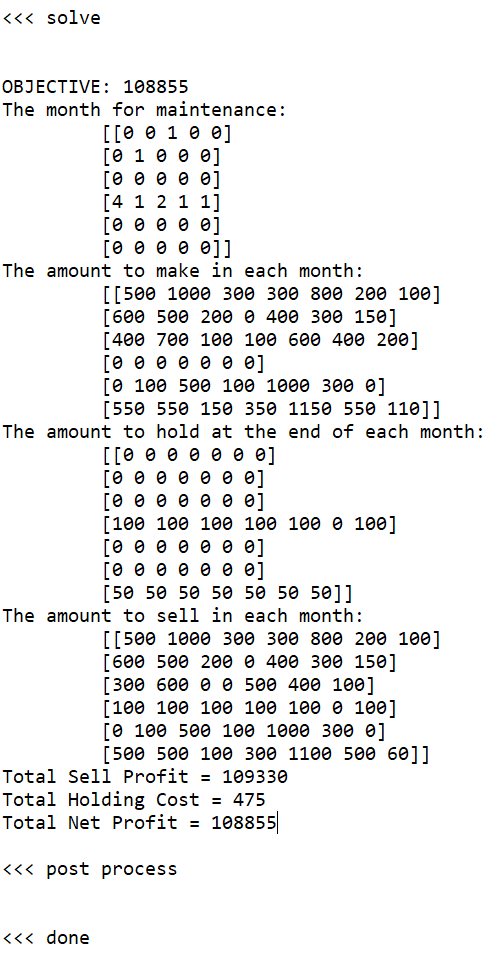
\includegraphics[width=0.5\textwidth]{profit.png}
    \caption{The result of \textit{CPLEX}}
\end{figure}

So we can answer the questions:

\begin{enumerate}
\item
\begin{enumerate}
\item The number of machine down for maintenance in each month:

\begin{table}[htbp]
      \scriptsize
      \centering
      \renewcommand\arraystretch{1.1}
      \begin{tabular}{m{0.1\textwidth} m{0.07\textwidth}<{\centering} m{0.07\textwidth}<{\centering} m{0.07\textwidth}<{\centering} m{0.07\textwidth}<{\centering} m{0.07\textwidth}<{\centering} }
      \hline
       & \textbf{grinder} & \textbf{vertical drill} & \textbf{horizontal drill} & \textbf{borer} & \textbf{planer}  \\\hline
      January & 0 & 0 & 1 & 0 & 0  \\
      February & 0 & 1 & 0 & 0 & 0  \\
      March & 0 & 0 & 0 & 0 & 0  \\
      April & 4 & 1 & 2 & 1 & 1  \\
      May & 0 & 0 & 0 & 0 & 0  \\
      June & 0 & 0 & 0 & 0 & 0 \\
      \hline
      \end{tabular}
    \end{table}
\end{enumerate}

\item
\begin{enumerate}
\item The amount to make for each product in each month:

    \begin{table}[htbp]
      \scriptsize
      \centering
      \renewcommand\arraystretch{1.1}
      \begin{tabular}{m{0.18\textwidth} m{0.07\textwidth}<{\centering} m{0.07\textwidth}<{\centering} m{0.07\textwidth}<{\centering} m{0.07\textwidth}<{\centering} m{0.07\textwidth}<{\centering} m{0.07\textwidth}<{\centering} m{0.07\textwidth}<{\centering}}
      \hline
       & \textbf{PROD 1} & \textbf{PROD 2} & \textbf{PROD 3} & \textbf{PROD 4} & \textbf{PROD 5} & \textbf{PROD 6} &  \textbf{PROD 7} \\\hline
      January & 500 & 1000 & 300 & 300 & 800 & 200 & 100 \\
      February & 600 & 500 & 200 & 0 & 400 & 300 & 150 \\
      March & 400 & 700 & 100 & 100 & 600 & 400 & 200 \\
      April & 0 & 0 & 0 & 0 & 0 & 0 & 0 \\
      May & 0 & 100 & 500 & 100 & 1000 & 300 & 0 \\
      June & 550 & 550 & 150 & 350 & 1150 & 550 & 110 \\
      \hline
      \end{tabular}
    \end{table}

\item The amount to sell for each product in each month:
	\begin{table}[htbp]
      \scriptsize
      \centering
      \renewcommand\arraystretch{1.1}
      \begin{tabular}{m{0.18\textwidth} m{0.07\textwidth}<{\centering} m{0.07\textwidth}<{\centering} m{0.07\textwidth}<{\centering} m{0.07\textwidth}<{\centering} m{0.07\textwidth}<{\centering} m{0.07\textwidth}<{\centering} m{0.07\textwidth}<{\centering}}
      \hline
       & \textbf{PROD 1} & \textbf{PROD 2} & \textbf{PROD 3} & \textbf{PROD 4} & \textbf{PROD 5} & \textbf{PROD 6} &  \textbf{PROD 7} \\\hline
      January & 500 & 1000 & 300 & 300 & 800 & 200 & 100 \\
      February & 600 & 500 & 200 & 0 & 400 & 300 & 150 \\
      March & 300 & 600 & 0 & 0 & 500 & 400 & 100 \\
      April & 100 & 100 & 100 & 100 & 100 & 0 & 100 \\
      May & 0 & 100 & 500 & 100 & 1000 & 300 & 0 \\
      June & 500 & 500 & 100 & 300 & 1100 & 500 & 60 \\
      \hline
      \end{tabular}
    \end{table}
    
\item The amount to hold for each product at the end of each month:
\begin{table}[H]
      \scriptsize
      \centering
      \renewcommand\arraystretch{1.1}
      \begin{tabular}{m{0.18\textwidth} m{0.07\textwidth}<{\centering} m{0.07\textwidth}<{\centering} m{0.07\textwidth}<{\centering} m{0.07\textwidth}<{\centering} m{0.07\textwidth}<{\centering} m{0.07\textwidth}<{\centering} m{0.07\textwidth}<{\centering}}
      \hline
       & \textbf{PROD 1} & \textbf{PROD 2} & \textbf{PROD 3} & \textbf{PROD 4} & \textbf{PROD 5} & \textbf{PROD 6} &  \textbf{PROD 7} \\\hline
      January & 0 & 0 & 0 & 0 & 0 & 0 & 0 \\
      February & 0 & 0 & 0 & 0 & 0 & 0 & 0 \\
      March & 100 & 100 & 100 & 100 & 100 & 0 & 100 \\
      April & 0 & 0 & 0 & 0 & 0 & 0 & 0 \\
      May & 0 & 0 & 0 & 0 & 0 & 0 & 0 \\
      June & 50 & 50 & 50 & 50 & 50 & 50 & 50 \\
      \hline
      \end{tabular}
    \end{table}
    
    
\end{enumerate}

\item The total selling profit is equal to \pounds109330.
\item The total holding cost is equal to \pounds475.
\item The total net profit is equal to \pounds108855.
\end{enumerate}
    \end{enumerate}
    \end{solution}
\end{enumerate}



\end{document}
